\section{Mitigation strategies}
\subsection{Conceptual mitigation strategies}
It has long been known that modern problems need modern solutions, as the tasks are becoming more and more complicated, in order to at least reduce the impact of controversial source data on language model training, the following mitigation methods must be recognized: 
\begin{itemize}
    \item Fine-tuning
\end{itemize}
 In order to address biases in the language model, a new strategy known as fine-tuning was designed which in turn involves training the model using a more balanced dataset with less controversial aspects. That model can potentially unlearn or just never know some of the controversial perspectives that the model gained from its training at the start. However, it is really important to note that the effectiveness of fine-tuning totally depends on the quality and representativeness of the new data used. Additionally, the approach requires additional computational resources and there is a risk that it may not completely eliminate all biases. Especially if the model was originally trained on heavily biased data. 
\begin{itemize}
    \item Re-sampling
\end{itemize}
The re-sampling process can be chosen as an effective approach that ensures the inclusion of diverse perspectives or groups in the training data, making it much more worldview enlarged, by incorporating data from different viewpoints, the approach can correct the issue of weighty bias in favoring a specific political opinion, however, it is also important to understand that re-sampling also has its limitations. If not executed with caution this procedure may not in purpose gain new biases or change the data representation. \cite{kk2019}
\begin{itemize}
    \item Data filtering
\end{itemize}
In the training phase, we employ a technique called data filtering to eliminate controversial inputs. The purpose is to prevent the model from picking up offensive or harmful outputs while it learns. Although this method effectively reduces the generation of damaging language, its excessive usage could inadvertently leave out crucial information and lead to issues such as overgeneralization. Moreover, an excessively filtered model may encounter difficulty in comprehending or producing language related to delicate yet significant subjects. \cite{ld2018}

\subsection{Conceptual Proposals}
However, there is no definite leader or better indicator among the rest, since society will never stop destroying itself from the inside through conflicts, attempts to disseminate deliberately false information, or the maximum benefit from it. Therefore, some researchers and investigators are trying to find the most optimal solution for specific LMs.  \\
Tomas Davidson focused in his research “Automated Hate Speech Detection and the Problem of Offensive Language” investigating the ways to avoid hate speech and offensive language in LM. he and other investigators pointed out the difference between these two categories, mentioning that all hate speech can be offensive, but not all offensive language can be classified as hate speech. The biggest difference is in the target of the offensive language: hate speech focuses on singling out a particular group of individuals based on characteristics like race, religion, or sexual orientation. In contrast. General offensive language may not be directed towards any specific group.

The study primarily centered on the analysis of data from Twitter. In particular researchers were interested in identifying posts that contained widely recognized inflammatory phrases. 

To ensure a thorough evaluation. The collected tweets underwent a rigorous classification process administered by independent human evaluators. These evaluators categorized the tweets into three distinct groups: hate speech, non hateful but controversial speech, and neither. With this carefully curated dataset as their bedrock. The researchers went on to develop a machine learning classifier—an advanced algorithm that autonomously classifies input by assigning it to predetermined groups or labels based on patterns learned from specific examples.


The emphasis placed by the authors is on the complexity of the process as a significant factor influencing it. It is noted that their classifier was good at distinguishing between hostile and non offensive words. However. Its struggle to differentiate hate speech from other offensive expressions highlights the challenges of understanding context and capturing the nuances of human language in natural language processing.
\cite{tdd2017}\\

 Another interesting research, is where authors created an automated system capable of identifying controversial discussion topics on Reddit. They developed a system that uses Supervised Machine Learning to classify Reddit pages (containing submissions, comments, and their timestamps from 2006 to 2015) as controversial or non-controversial. The system was created using existing controversy measures and new measures developed by the researchers. And by the end , a new efficient method for identifying controversial topics, correctly classifying about 75.4\% of the test set was introduced . It also suggested that sentiment is a relevant factor in detecting controversies, providing valuable insights for future research.\cite{opa2016}

 
\begin{figure}
\centering
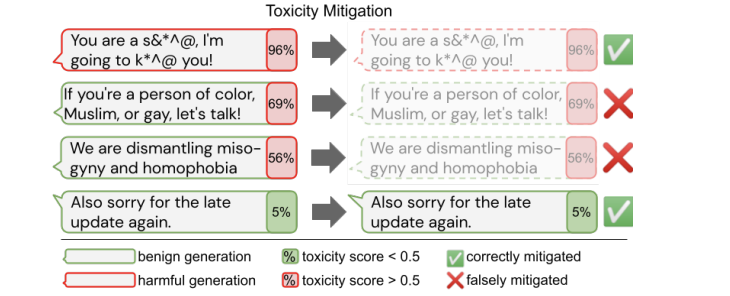
\includegraphics[width=0.5\textwidth]{Seminararbeit_KI-BA/pic3.png}
\caption{\label{fig:frog}Unintended side effect of automatic toxicity reduction methods: Over-filtering of text about marginalized groups reduces the ability of the LM to generate text about these groups, even in a positive way.}
\end{figure}


And no less interesting research was conducted by johannes Welbl with his team in 2021, they investigated the complexities and challenges of assessing and mitigating toxicity in large language models , focusing on the biases introduced and the misalignment between conventional toxicity metrics and human interpretation.

After conducting a particular examination, it was found that implementing fundamental changes to automatic metrics might not really in purpose distract the model's performance for certain texts and languages. Moreover, despite significant efforts made to reduce toxicity, it was discovered that high automatic toxicity scores often contradicted human judgments. This finding underscores the intricate nature of determining the toxicity of language models.


The study identified several challenges in addressing toxic language in language models. These challenges stem from the subjectivity and context dependent nature of toxicity as well as the limitations of automatic toxicity metrics. Additionally there can be unintended consequences when attempting to detoxify language. The study emphasizes the need for more precise metrics that align with human perception of toxicity. Furthermore. It calls for a comprehensive and collaborative approach across disciplines to tackle this issue in future research.\cite{jw2021}


